\newpage
\section{Project Documentation}
Below you will find everything that is required in order to run our project.
First, you will find a list of all the materials used in our project.
Next, you will find a list of steps and images describing the process to setup the hardware along with a block diagram explaining the connections between devices.
The following two sections will list our projects dependencies along with instructions to program the microcontroller.
Lastly, a step has been included for running our project and verifying the results. \\

\subsection*{Required Hardware}
\begin{itemize}
\item{2x SparkFun IMU Breakout - MPU-9250}
\item{Adafruit Metro Mini 328 -5V 16MHz}
\item{PC /w display}
\item{USB 2.0 cable - Type-A Male to Mini Type-B Male}
\item{2x breadboard}
\item{Wires to connect MPUs and Microcontroller}
\item{Solder}
\item{Soldering Iron}
\item{Male Headers to connect devices to breadboard}
\end{itemize}

\subsection*{Hardware setup}
\begin{itemize}
\item{Modify Microcontroller to output 3.3v on its digital logic pins \\ 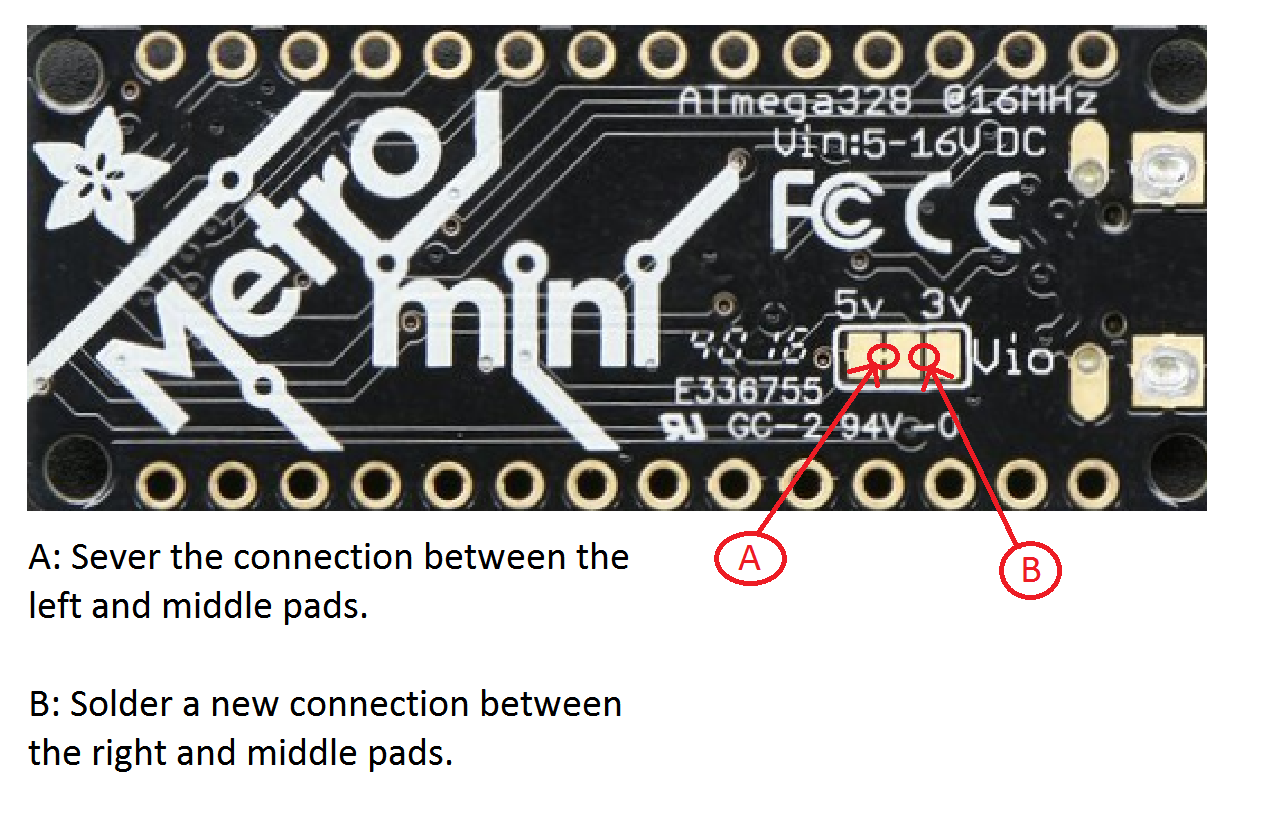
\includegraphics[scale=0.5]{mm_mod}}
\item{Modify IMUs to allow their AD0 pins to receive voltage which enables dynamic I2C addresses \\ 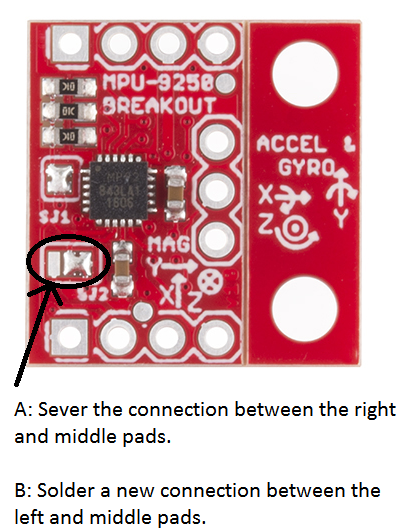
\includegraphics[scale=1.5]{mpu_mod}}
\item{Solder male headers to the bottom of the microcontroller}
\item{Solder male headers to the bottom of both IMUs}
\item{Attach the microcontroller and one IMU to the first breadboard}
\item{Attach the second IMU to the second breadboard}
\item{Connect devices and pc \\ 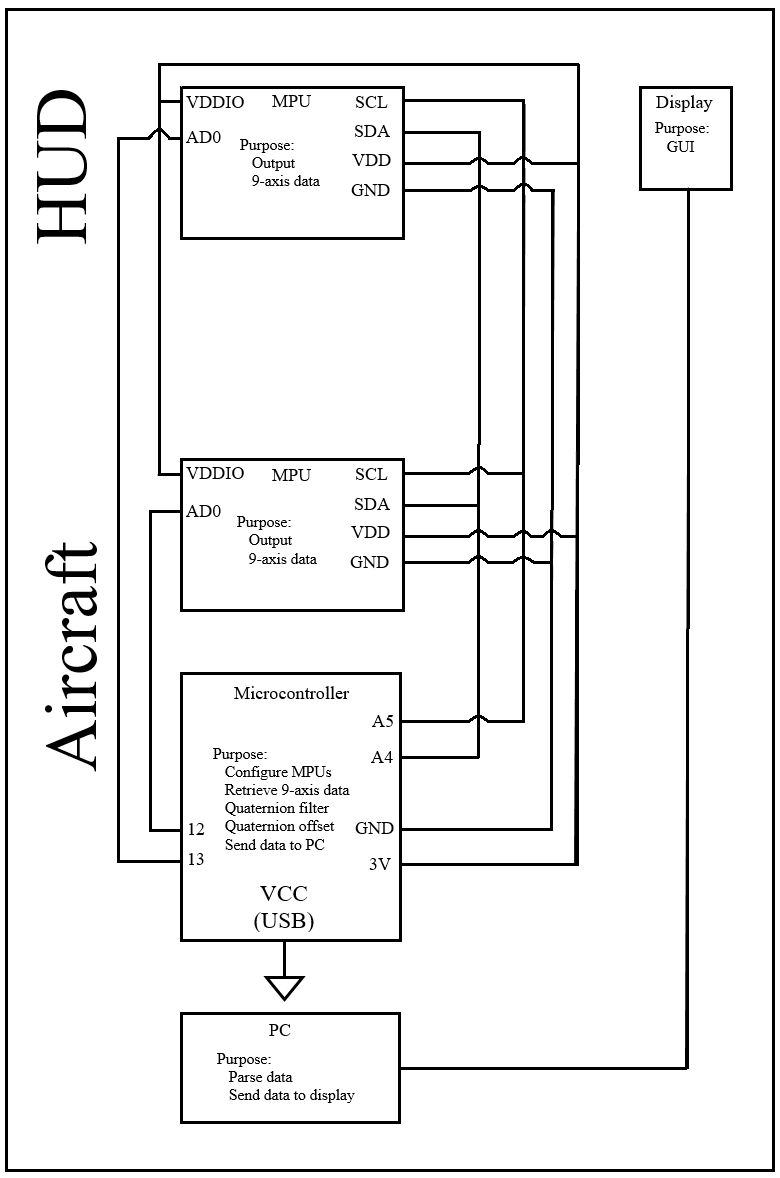
\includegraphics[scale=0.75]{Block_Diagram}}

\end{itemize}

\subsection*{Setup Dependencies}
\begin{itemize}
\item{Install the Arduino IDE}
\item{Install Python 2.7.9}
\item{Install VPython}
\item{Install pySerial}
\item{Download our arduino project}
\item{Download our python script}
\end{itemize}

\subsection*{Program Hardware}
\begin{itemize}
\item{Ensure that the microcontroller is connected to the PC}
\item{Load our arduino project on the Arduino IDE}
\item{Program the microcontroller with our project through the Arduino IDE}
\end{itemize}

\subsection*{Run application}
\begin{itemize}
\item{Load our python script}
\item{Run the script and follow instructions}
\item{Verify results by viewing the GUI}
\end{itemize}

\subsection*{PSEUDO CODE}
\begin{lstlisting}
// Place HUD in alignment with aircraft IRU
wait()
 
// Setup:
for each MPU-9250:
	update AD0 pin	// Do this in order to change I2C address
	initialize/configure registers
	for each sensor: // Accelerometer, Gyroscope, and magnetometer
		initialize/configure registers
calibrate device
 
// Install HUD
wait()
 
// Static Offset Mode
while statistical confidence insufficient:
	while sample size insufficient:
		for each MPU-9250:
			read data
			update stored quaternion value via quaternion filter
		record quaternion offset sample
	perform confidence interval
 
send static offset via serial port
 
// Dynamic offset mode
while system is active:
for each MPU-9250:
	read data
	update stored quaternion value via quaternion filter
record quaternion offset
 
send dynamic offset via serial port
\end{lstlisting}